\chapter{Background}
\label{ch:background}

\section{Cellular Automata}
Cellular Automata (CA) are an array of cells capable of holding different states. The array can then be iterated by applying a rule set to each cell resulting in a new state being set. These rules take the cell’s current state and its neighbour’s states as inputs and then defines what the next state should be. CA were first used by von Neumann for his 29 state "universal constructor" in 1966 \cite{VONNEUMANN1966}.

One of the simplest examples of CA are called elementary cellular automaton and were extensively studied by S. Wolfram \cite{WOLFRAM2002}. These are one\mbox{-}dimensional, binary, nearest neighbour CA. A one\mbox{-}dimension array is used to hold the state of cells which can either be 1 or 0. The rules to update these cells use the two nearest neighbours to the cell and its current state to calculate the next state. This make 3 inputs to the rule giving a total eight possible input states. These input states can either be assigned to output 1 or 0 giving 256 possible forms of the elementary CA. Figure \ref{fig:CODE30} shows an example rule set for this type of automaton, known as Rule 30. The diagram at the top shows every possible combination of the 3 inputs, centre cell and two nearest neighbours, and the output to that assigned pattern. This is known as Rule 30 due to the binary value made by the outputs. The grid below shows the effect this rule has when implemented on the row above. The top row at the top is the initial state and each row down is an iteration of the CA. These simple rules can lead to very useful CA with Rule 30 being used for random number generation and Rule 184 for traffic modelling.

\begin{figure}[h]
	\centering
	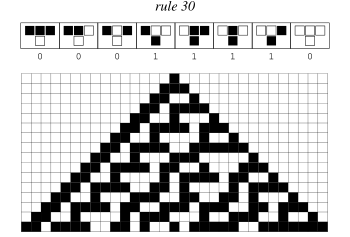
\includegraphics[width=0.8\textwidth]{ElementaryCARule030_700.png}
	\caption{Rule 30 and its iterations \cite{WOLFRAMCODE}}
	\label{fig:CODE30}
\end{figure}

Another example of CA is Conway’s Game of Life (CGOL) \cite{GARDNER1970} which uses a two\mbox{-}dimensional array of binary cell’s but with a totalistic rule set meaning the average of neighbours is used. CGOL uses the Moore neighbourhood, square of closest neighbours to cell, with the following rules to determine the cells next state.

\begin{enumerate}
	\item Set state to 0 if sum of Moore neighbours is less than 2 or greater than 3.
	\item Set state to 1 if sum of Moore neighbours is 2 or 3 and current state is 1.
	\item Set state to 1 if sum of Moore neighbours is 3 and current state is 0.
\end{enumerate}

When calculating the next iteration of CA the rules are applied independently to each cell creating an inherently parallel process. This creates an excellent opportunity to use a hardware accelerator to exploit this parallelism allowing for any size CA to be computed in constant time if a sufficiently large accelerator is used.

\subsection{Applications}
CA have many real world applications such as modelling physical or chemical systems. One useful application is simulating forest fires \cite{MUTTHULAKSHMI2020}. This simulation can then be used to test how effective various fire fighting strategies are and plan responses for future forest fires. Another use case is traffic modelling. Rule 184 is a particularly useful basis for this as it models traffic jams in a one dimensional stream. The Biham, Middleton and Levine Model extends this to act in two dimensions and can then be applied to predict real time traffic jams \cite{HU2017}.

\section{FPGAs}
A Field Programmable Gate Array (FPGA) is a semiconductor device based around a matrix of Configurable Logic Blocks (CLB), Input/Output Blocks and specialized blocks such as for Digital Signal Processing (DSP) \cite{XILINXARCH}. Logic can take two forms, combinatorial and behavioural. Combinatorial logic takes in a set of new input and based on a set of rules determines the output. Behavioural logic takes in new input but also uses previous outputs to determine what the next output is. To achieve this, data must be stored for use in future computations. CLB use Lookup Tables (LUT) for combinatorial logic and Flip\mbox{-}Flops (FF) to store values for behavioural logic. A LUT is a small memory block where the inputs are used to address a bit of memory and the values stored there represents the output of the logic. Any truth table can be stored in these LUTs and if more inputs are required multiple LUTs can be combined. Figure \ref{fig:CLB} shows the structure of a CLB.

\begin{figure}[h]
	\centering
	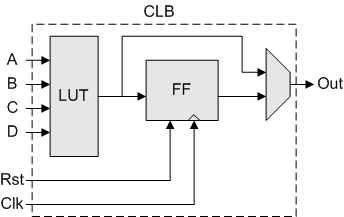
\includegraphics[width=0.7\textwidth]{CLB_Block_Diagram.png}
	\caption{Block diagram of a CLB \cite{FPGAKEY}}
	\label{fig:CLB}
\end{figure}

While CLB could achieve any task, they sacrifice efficiency for adaptability. So some very common and useful functions are given dedicated blocks such as the DSP which allows for operations such as addition and multiplication to be completed with greater efficiency. Blocks are connected together through configurable switches allowing signals to take any route through the blocks. This structure is show in Figure \ref{fig:FPGASTRUCT}.
\newpage
The ability to program the FPGA to act as any hardware makes it an excellent solution for rapid development of hardware as new designs can be tested and iterated on without incurring any additional costs. For this project a Xilinx Nexys A7 100T development board was used.

\begin{figure}[H]
	\centering
	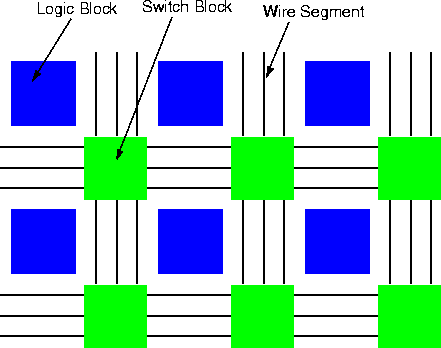
\includegraphics[width=0.6\textwidth]{fpgastruct.png}
	\caption{Structure of an FPGA block matrix with configurable routing \cite{FPGAARCH}}
	\label{fig:FPGASTRUCT}
\end{figure}

\subsection{Verilog}
FPGAs are programmed using a Hardware Description Language (HDL) which describes the logic that is run. This project uses Verilog as it is a relatively low level HDL giving fine control over the implemented design. Verilog code can then be synthesised into a form that optimises the logic for use on FPGAs in general. It can then be implemented for the specific FPGA used and mapped onto the cells inside the FPGA. As a Xilinx FPGA is used in this project the Vivado Design Suite 2023.2 was used to perform these steps.

\section{RISC\mbox{-}V}
As an open standard ISA, RISC\mbox{-}V provides a royalty free base that can be used when creating custom solutions which require a processor. This guarantees the design will function with the plethora of publicly available software and tools designed for RISC\mbox{-}V processors reducing the work required to get a fully functional product. These tools include a RISC\mbox{-}V GNU Compiler Toolchain with GCC for compiling C code \cite{RISCVGNU} and a port of Debian \cite{DEBIANRISCV}. The RISC\mbox{-}V GNU Compiler Toolchain will be particularly useful for this project as it will be used to compile bare\mbox{-}metal code. RISC\mbox{-}V’s open nature and compatibility has led to wide spread adoption with an estimated shipments of RISC\mbox{-}V based System\mbox{-}on\mbox{-}chip (SoC) at 16.2B units in 2030, with revenues reaching \$92B \cite{SHDGROUP}.

\subsection{Rocket Chip}
Rocket Chip is an open\mbox{-}source SoC generator that uses the RISC\mbox{-}V ISA \cite{Asanović:EECS-2016-17}. This tool can be used to configure and generate a RISC\mbox{-}V SoC into synthesizable RTL for use on FPGAs. A second project called vivado\mbox{-}risc\mbox{-}v uses Rocket Chip to generate a set of cores that are directly compatible with the Nexys A7\mbox{-}100T FPGA board used in this project \cite{VIVADORISCV}. It also provides scripts and documentation to setup and run the Linux kernel and compile bare\mbox{-}metal code. In its current state the bootable Linux environment this project creates has many issues, the biggest being exceedingly long boot times. However, it should be possible to add the custom hardware created in this project as a preferential in the device tree allowing for its use within Linux.

\subsection{AXI}
The Advanced eXtensible Interface (AXI) is a royalty\mbox{-}free communication bus protocol that is part of the ARM Advanced Microcontroler Bus Architectrue (AMBA) standard \cite{AMBAAXI}. The AXI protocol has been adopted by Xilinx for use with FPGA IP block designs \cite{XILINXAXI} and is common in many other SoCs. There are 3 interfaces: AXI4, AXI4\mbox{-}Lite and AXI4\mbox{-}Stream. AXI4 provides high\mbox{-}performance memory\mbox{-}mapped communication and AXI4\mbox{-}Stream allows for high\mbox{-}speed streaming of data. For this project, AXI4\mbox{-}Lite will be used as it is a simpler interface for low\mbox{-}throughput memory\mbox{-}mapped communication. AXI4\mbox{-}Lite uses five channels. Two for read transactions consisting of address and data and three for write transaction which uses an additional write response channel \cite{REALDIGITAL1}. The AXI4 specification uses a VALID/READY handshake to allow both the master and slave to control the transfer rate. The VALID signal is set when the address or data is ready to be sent and the READY signal is set when the destination is ready to accept the data. The transaction completes when both signals are set during a rising clock edge. Figures \ref{fig:AXIREAD} and \ref{fig:AXIWRITE} shows the activity of the signals used in AXI read and write transactions. These show the handshake being performed and data getting transferred.

\begin{figure}[h]
	\centering
	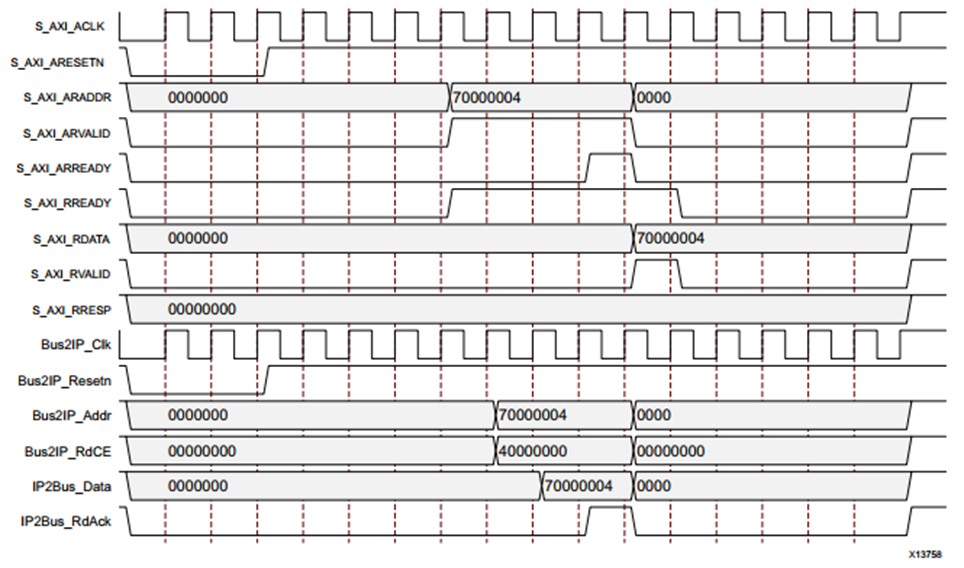
\includegraphics[width=0.8\textwidth]{axiread.png}
	\caption{Signals used in AXI read transactions \cite{REALDIGITAL1}}
	\label{fig:AXIREAD}
\end{figure}

\begin{figure}[h]
	\centering
	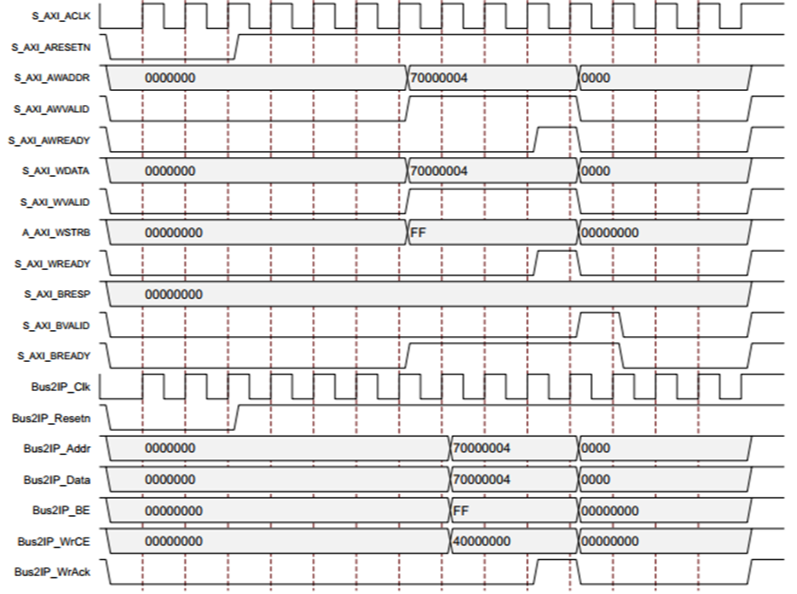
\includegraphics[width=0.8\textwidth]{axiwrite.png}
	\caption{Signals used in AXI write transactions \cite{REALDIGITAL1}}
	\label{fig:AXIWRITE}
\end{figure}

\chapter{Related Works}
\section{Implementation of a RISC\mbox{-}V Processor with Hardware Accelerator}
This paper covers the development of a hardware matrix multiplier for a RISC\mbox{-}V processor. A ZedBoard development board, using the same Artix\mbox{-}7 FPGA chip as the Nexys A7\mbox{-}100T, is used. The RISC\mbox{-}V core used in this project is generated by PULPino which creates a 32\mbox{-}bit, single\mbox{-}core microprocessor \cite. This is a simpler core and requires less FPGA resources to implement, freeing more space for custom hardware. Our project uses a 64\mbox{-}bit core generated with Rocket Chip which reduces the available resources. However, due to the configurability of Rocket Chip the core can be changed to a smaller 32\mbox{-}bit core if needed.They used the APB bus to communicate between the accelerator and PULPino microprocessor due to its interface being simpler than the AXI bus. In our project, the AXI interface will be used as it provides the option for higher\mbox{-}performance transfers and is more often used when connecting internal hardware. When tested their accelerator reduced the number of clock cycles required from 603 to 134. This is a good improvement but due to the processor having a clock speed of 5 MHz, it is unable to compete with modern processors. They encountered many errors when trying to build C programs for the PULPino and required much trial and error. The process of compiling code in our project has proved to be far simpler.

\section{Design and Implementation of Cellular Automata on FPGA for Hardware Acceleration}
This project implements an accelerator for Conway’s Game Of Life. They use a DE1\mbox{-}SoC development board with a Cyclone V FPGA chip. Their design uses a lattice of cell modules that read the neighbours states from a register file and write their next state back to it. Our design is similar in its use of a board register but to provide more adaptability all cells states are sent to each cell rather than only the 8 neighbours. This allows the cell to use any neighbourhood. They also include the load state function in the cell module using a multiplexer in the same way as our design. They integrate a mouse and VGA controller into their design to allow for control and result output. Another feature implemented is a save manager that stores previous board states. A similar feature to this could be added to our design to allow intermediate states to be pulled as required while the accelerator continues to compute removing the need to wait for each one. Their design achieved a speed boost of 36.7x against a GPU implementation and 2908x against a software implementation. This shows the benefit of accelerators such as even when compared to modern GPU parallelization.

\section{Cellular Automata Hardware Implementations - an Overview}
This paper explains the requirements for general cellular automata hardware that should be able to implement any local rule. It then reviews the methods this hardware could be implemented. FPGAs can be reconfigured to fit a particular CA from a hardware description. A programmable cellular automata allows the same hardware to be used for any local rule. This form of general cellular automata has been implemented on FPGAs by the University of Porto (Portugal) \cite. Cellular automata machines are a different approach which use pipelined serial processing. Finally it mentions the uses of systolic arrays for parallel processing of CA.